

\documentclass[english]{article}
\usepackage[T1]{fontenc}
\usepackage[latin9]{inputenc}
\usepackage{listings}
\usepackage{graphicx}
\usepackage{amsfonts}

\makeatletter

\newcommand{\noun}[1]{\textsc{#1}}

\makeatother

\usepackage{babel}
\begin{document}

\title{STNUM - TP1\\
LOGICIEL R ET RAPPEL DES PROBABILIT�S}


\author{\noun{Ma�lis Boudier}\\
\noun{Juste Raimbault}}

\maketitle

\section*{Question 1}

The command \texttt{rnorm} generates random numbers following a centered
gaussian law, for which the density is, if $\sigma$ is the standard
deviation, $f(x)=\frac{1}{\sqrt{2\pi\sigma^{2}}}\cdot e^{-\frac{1}{2}\cdot\frac{x^{2}}{\sigma^{2}}}$.
The maximal value taken is then $\frac{1}{\sigma\sqrt{2\pi}}$, and
therefore we fix the upper bound for $y$ just a little above this
value (1.2 times, taking the maximum with the frequencies of the histogram,
since the bars can go above the theoretical curve), after having calculated
$\sigma$ by $\sigma=$ \texttt{sd(x)}.


\section*{Question 2}

See code for loading of data of geyser eruptions.

Command \texttt{summary(geyser)} gives basic informations about waiting
times between eruptions and duration of each eruption. Result are
presented in figure 1. Figure 2 presents the empirical distributions
and figure 3 histogram for both series.

\begin{figure}
\hfill{}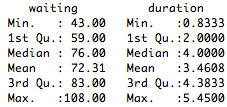
\includegraphics[scale=0.6]{geyser}\hfill{}

\caption{Basic statistical data for both series}


\end{figure}


\begin{figure}
\hfill{}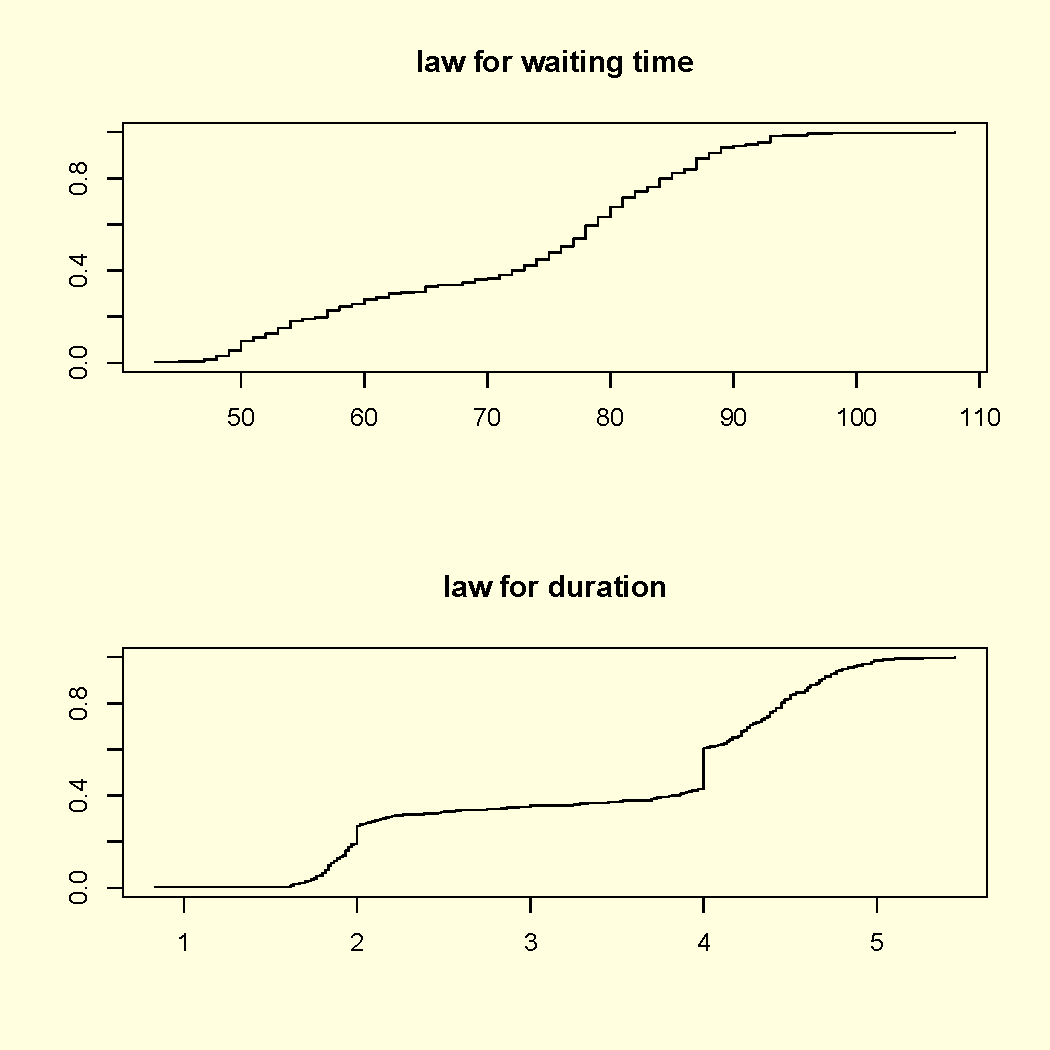
\includegraphics[scale=0.45]{geyserLaws}\hfill{}\hfill{}\caption{Empirical distributions}


\end{figure}


\begin{figure}
\hfill{}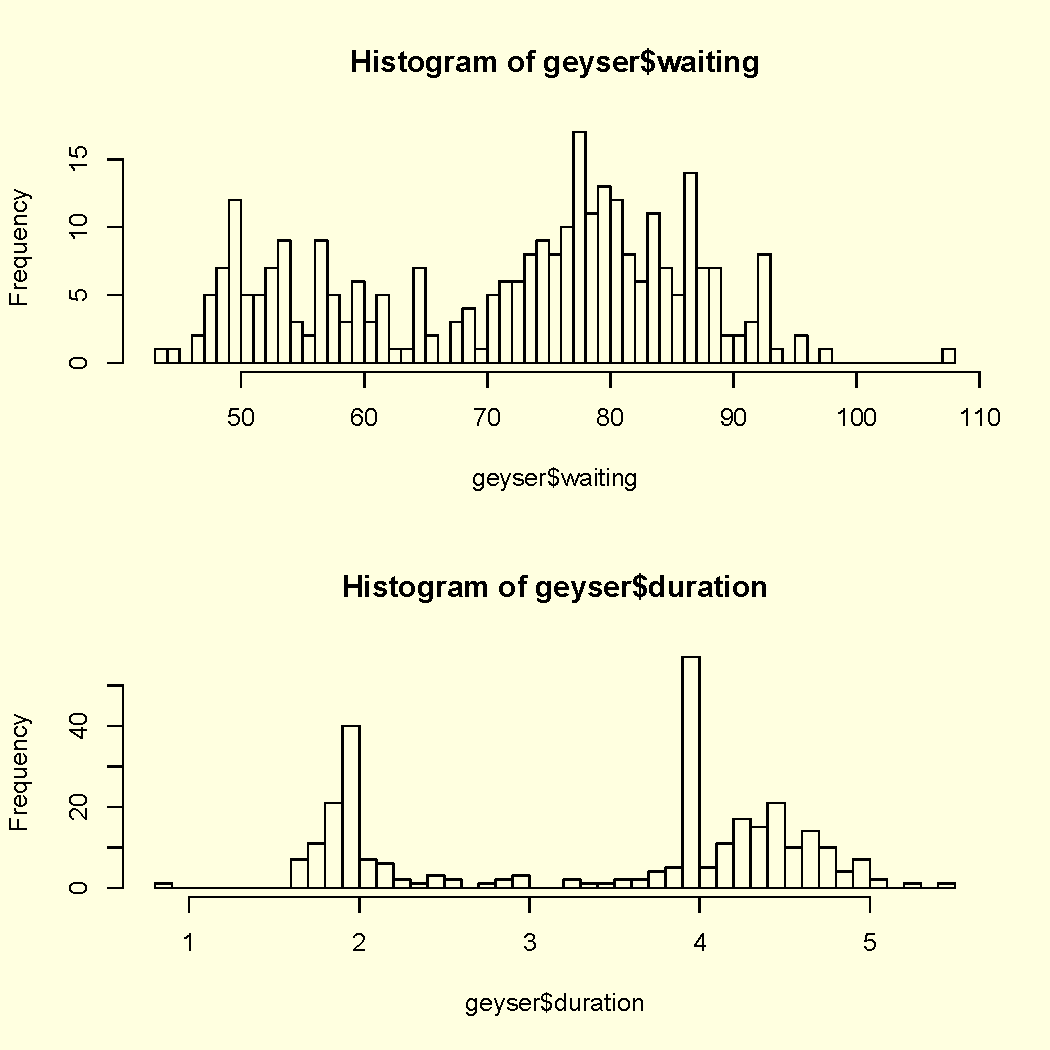
\includegraphics[scale=0.45]{geyserHist}\hfill{}\hfill{}\caption{Histograms for geyser waiting time and duration}


\end{figure}


\newpage{}


\section*{Question 3}

\begin{figure}
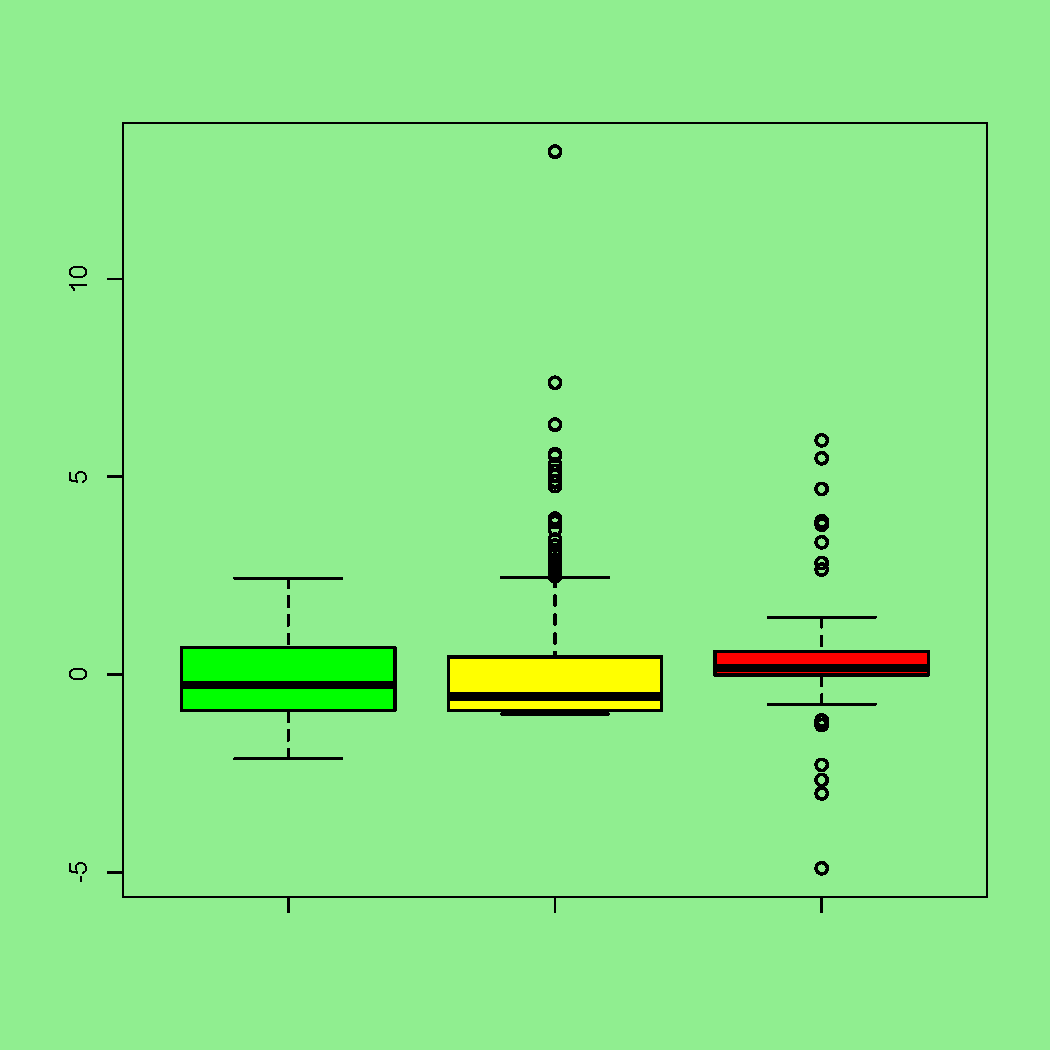
\includegraphics[scale=0.7]{boxplot35}\caption{Boxplots of 3.5}


\end{figure}


The parallel boxplots of 3.5 are presented in figure 4.


\paragraph{(a)}

The most dispersed distribution is the first one since dispersion
corresponds to the size of the box with tails (from A to B).


\paragraph{(b)}

The second distributions seems to have more outliers points than the
two others.


\section*{Question 4}


\paragraph{(a)}

The weight that such a proportion of cable can carry correponds to
the 3rd quartile, i. e. 12,25 T.


\paragraph{(b)}

The boxplot can be seen in figure 5. There is one outlier (point at
7), because it appears to be outside the standard values (and is therfore
represented that way). The value of the third quartile if the coordinate
of the upper bound of the box. 

\begin{figure}
\hfill{}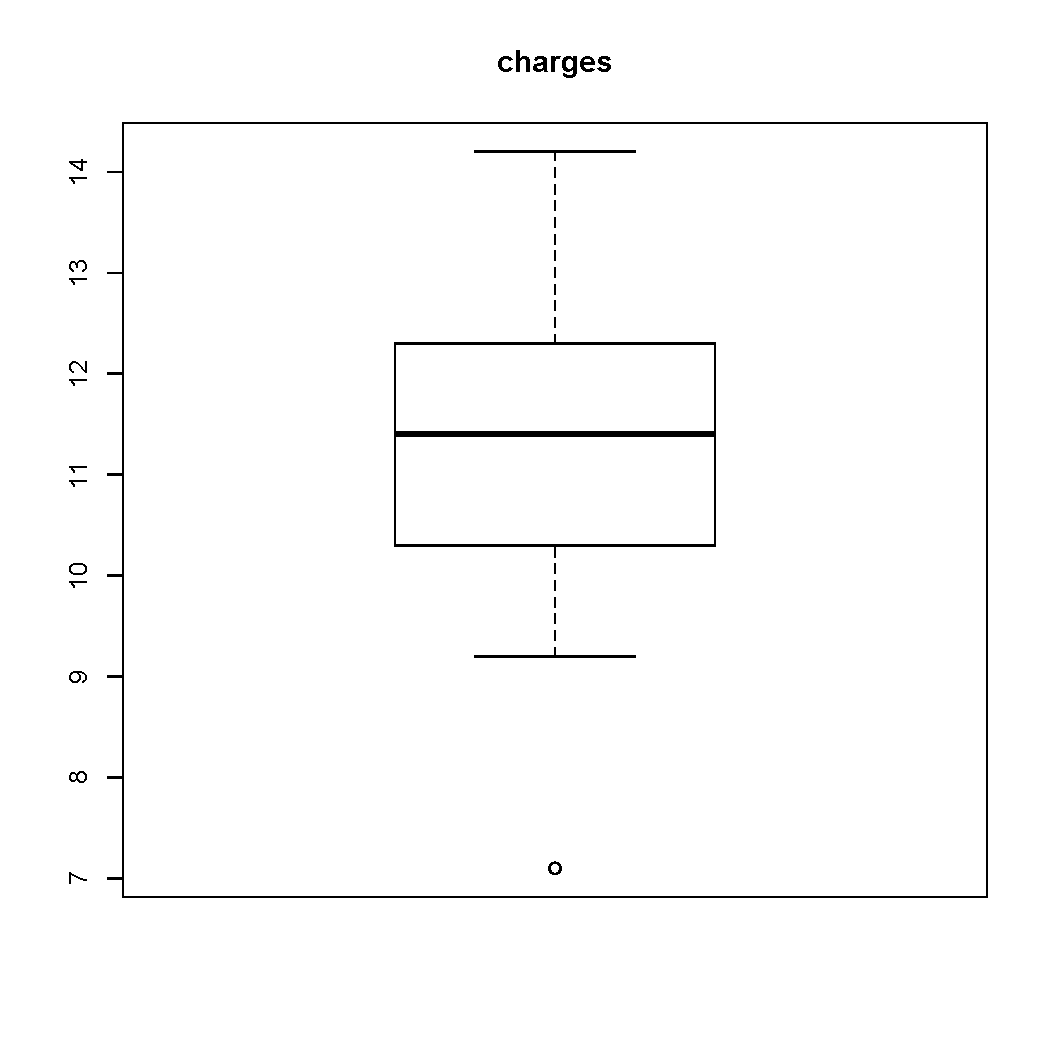
\includegraphics[scale=0.7]{charges}\hfill{}\hfill{}\caption{Boxplot for cables capacity data}


\end{figure}



\paragraph{(c)}

The parts of the box around the median are not of same size and the
tails are also of different sizes, so the distribution is not symmetric.


\section*{Question 5}

See code for graphic representation of empirical laws.


\paragraph{(i)}

Figure 5 shows superposition of empirical curve of the law of $T_{i}$
and the curve $1-exp(-x/2)$. The distribution function of $T_{i}$
should be that one since their shapes are very close.
One can find the result by calculations: $F_{T}(x)=\mathbb{P}(T<x)
=\mathbb{P}(-2ln(U)<x) =\mathbb{P}(U>exp(-x/2)) =1-\mathbb{P}(U\leq
exp(-x/2))=1-exp(-x/2)$, because $U$ is uniformaly distributed.

\begin{figure}
\hfill{}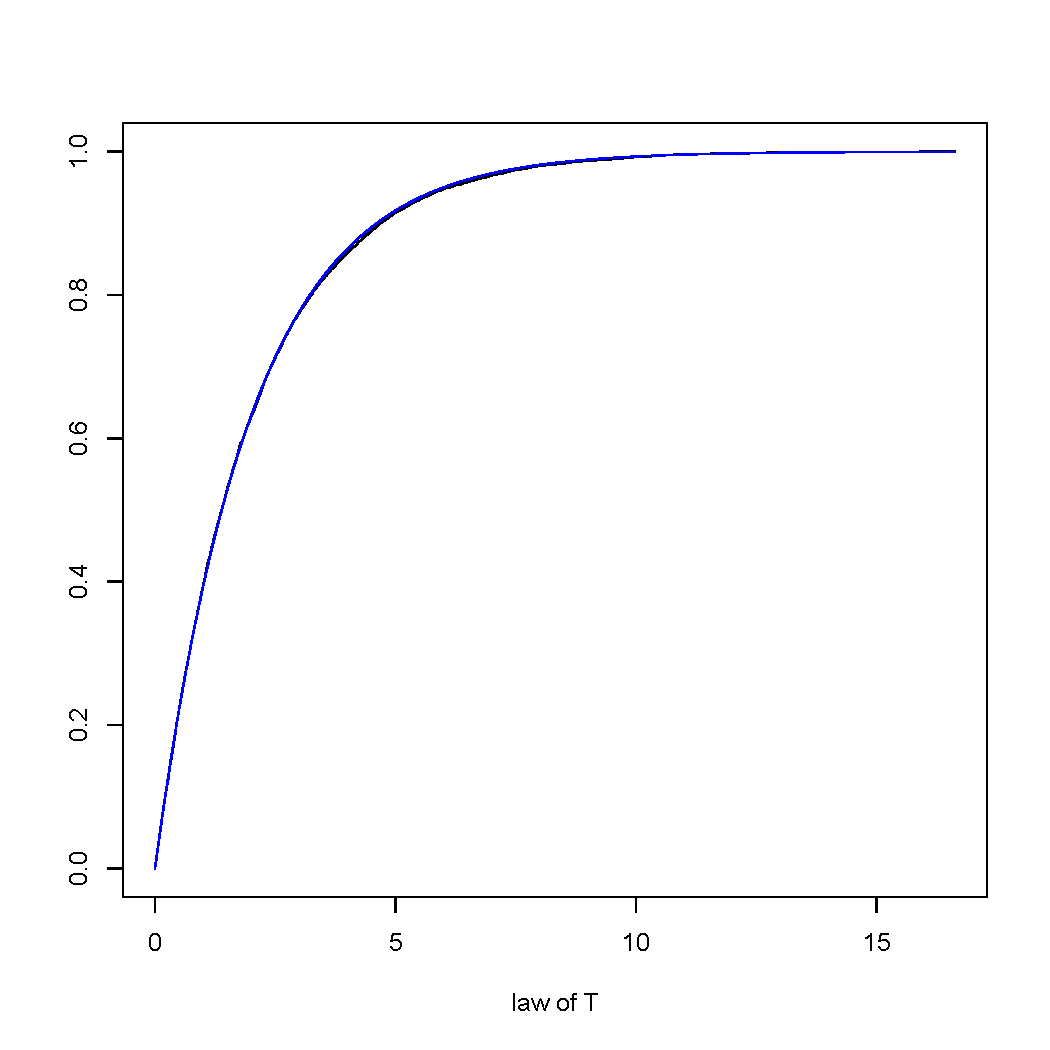
\includegraphics[scale=0.35]{lawT}\hfill{}\hfill{}\caption{Law of $T_{i}$}


\end{figure}



\paragraph{(ii)}

See figure 6. The law of $X_{i}$ seems to be not so far from the
function $\frac{1}{0.82*\pi}arctan(pi*x/2.3)+0,5$. The exact law can be
calculated by conditioning on $\sqrt(T)$ and is given by an integral.

\begin{figure}
\hfill{}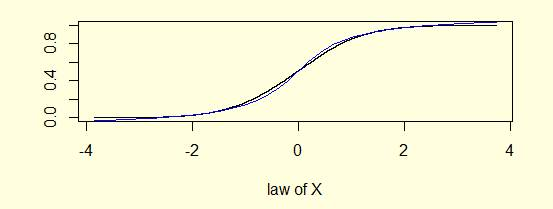
\includegraphics[scale=0.7]{lawX.jpg}\hfill{}\hfill{}\caption{Law of $X_{i}$}
\end{figure}


\newpage{}


\section*{Source code}

\begin{lstlisting}[basicstyle={\footnotesize},numbers=left,numberstyle={\footnotesize},stepnumber=5]
##STNUM - TP1

##Question 1
##see report

##Question 2
library(MASS)
data(geyser)

#Statistic description
summary(geyser)
#Distribution function
par(mfcol=c(2,1),bg="lightyellow")
n=length(geyser$waiting)
plot(sort(geyser$waiting), 1:n/n, type="s", ylim=c(0,1),
   xlab="", ylab="",main="law for waiting time")
n=length(geyser$duration)
plot(sort(geyser$duration), 1:n/n, type="s", ylim=c(0,1), 
   xlab="", ylab="",main="law for duration")
#Boxplots
par(mfcol=c(2,1),bg="lightyellow")
boxplot(geyser$waiting) 
boxplot(geyser$duration)
#histograms
par(mfcol=c(2,1),bg="lightyellow")
hist(geyser$waiting,breaks=50)
hist(geyser$duration,breaks=50)

##Question 3 
###see report

##Question 4
charges<-c(10.1,12.2,9.3,12.4,13.7,10.8,11.6,10.1,11.2,
  11.3,12.2,12.6,11.5,9.2,14.2,11.1,13.3,11.8,7.1,10.5)

##a 
summary(charges)
##The value of the 3rd quartile is 12.25

##b 
boxplot(charges,main="charges")

## Question 5
U = runif(10000,0,1) 
V = runif(10000,0,1) 
T = -2*log(U)
X = sqrt(T)*cos(2*pi*V)

#i : law of T ?
n=length(T)
plot(sort(T), 1:n/n, type="s", ylim=c(0,1), xlab="law of T", ylab="") 
curve(1-exp(-x/2),add=TRUE,col="blue",ylab="")
#ii : law of X
f<-function(x){1-area(function(v){0.5-atan(pi*x/2.3)/(0.82*pi)},0,1)}
n=length(X)
plot(sort(X), 1:n/n, type="s", ylim=c(0,1), xlab="law of X", ylab="")
curve(from = -5,to = 5,0.5+atan(x)/pi,add=TRUE,col="blue",ylab="")
\end{lstlisting}

\end{document}
